\documentclass[english]{article}
\usepackage[T1]{fontenc}
\usepackage[latin9]{inputenc}
\usepackage{babel}
\usepackage{graphicx}
\graphicspath{{images/}}
\begin{document}

\title{Specific Requirement}

\section{UseCase Diagram}

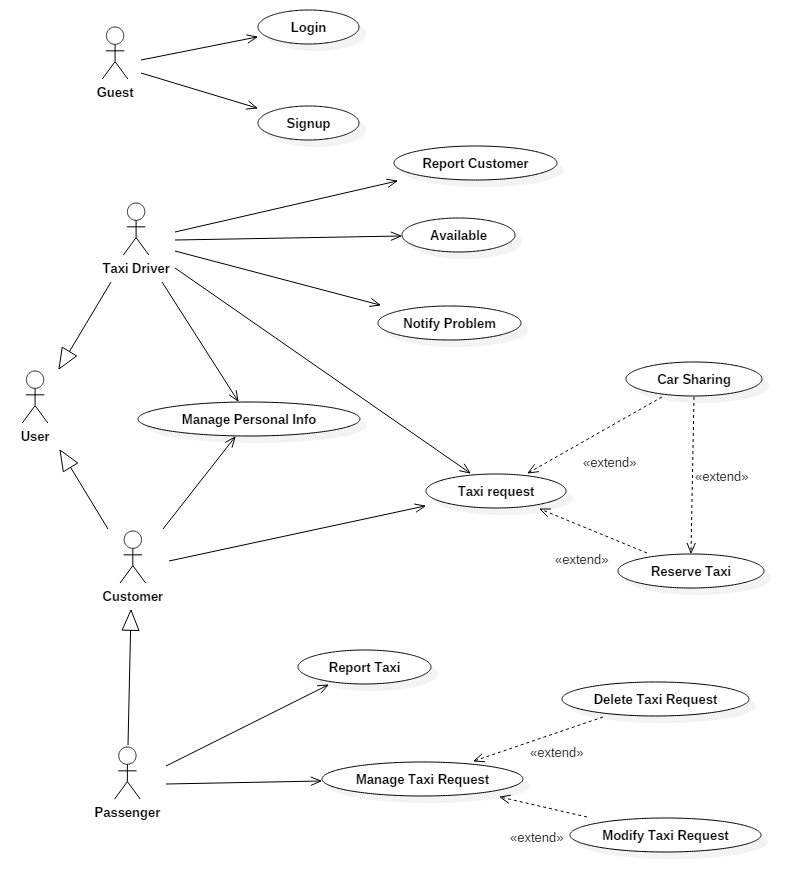
\includegraphics[width=\textwidth]{UseCase}

\section{Sequence Diagram}

\subsection{Signup}

\begin{tabular}{lp{8cm}}
\hline
Actors & Guest \\
\hline
Preconditions &  The Guest is not registered into the system \\
\hline
Execution Flow &  
		\begin{enumerate}
			\item The Guest request the registration page
			\item The System requires the Signup information
			\item The Guest fill the form and submit the request
			\item The System check the uniqueness of the Username and E-Mail
			\item The System create the User (or Taxi drive) profile
			\item The System send the confirm the the Guest
		\end{enumerate} 
	\\ 
\hline
Postconditions & The guest is now a User o a Taxi driver \\
\hline
Exceptions & The E-Maill or username are not unique or, in the case of taxi driver signup, the licenses are not valid
\end{tabular}

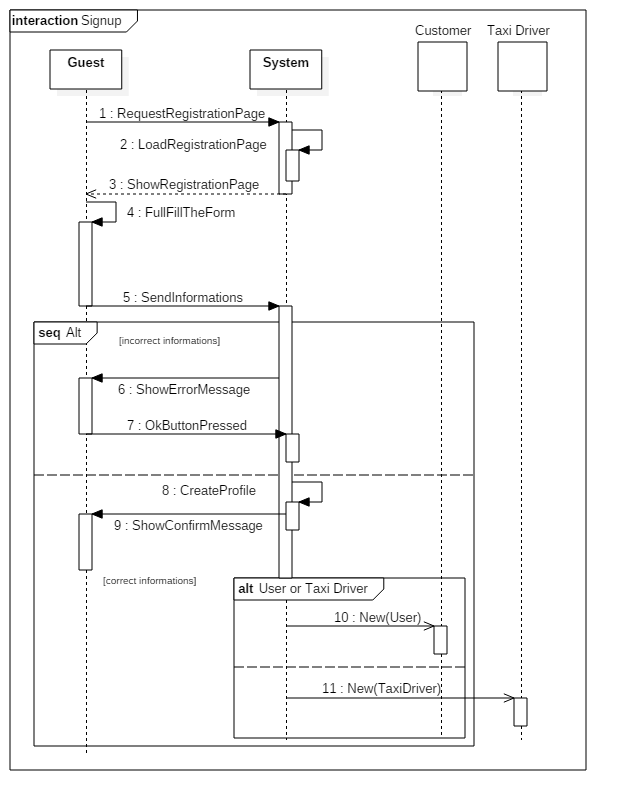
\includegraphics[width=\textwidth]{Signup}

\subsection{Login}

\begin{tabular}{lp{8cm}}
\hline
Actors & Guest \\
\hline
Preconditions &   The Guest has already a profile into the System\\
\hline
Execution Flow &  
		\begin{enumerate}
			\item The Guest request the login page
			\item The System requires the Login information (Username, Password)
			\item The Guest fill the form and submit the request
			\item The System check the Username and Password
			\item The System send the confirmation of Login
			\item The Guest is logged into the System
			\item The Guest is redirected to the User profile Page
		\end{enumerate} 
	\\ 
\hline
Postconditions & The guest is now a User or Taxi Driver \\
\hline
Exceptions & The Usename, password couple is incorrect, so the Guest cannot log in
\end{tabular}

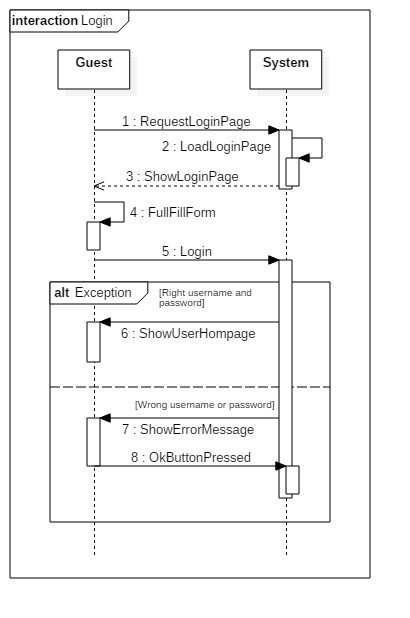
\includegraphics[width=\textwidth]{Login}

\subsection{Taxi Request}

\begin{tabular}{lp{8cm}}
\hline
Actors & User, Taxi Driver \\
\hline
Preconditions & The User should not be banned \\
\hline
Execution Flow &  
		\begin{enumerate}
			\item The Guest request the Taxi Request page
			\item The System requires the type of request the User wants to perform
			\item The User provide the choice to the System
			\item The System ask for the information to perform the choose request
			\item The User fill the form and send the information to the System
			\item The System forward the request to the first Taxi Driver of the local queue
			\item If the Taxi Driver answer positively to the request he take in charge the User, otherwise he deny the request
			\item If the Taxi Driver answered positively the System notify to the User the incoming taxi and change the availability of the Taxi Driver, otherwise the System update the queue and forward the request to the new first of queue until the queue is not repeated
			\item If there are no Taxis available the System notify to the User the unavailability
		\end{enumerate} 
	\\ 
\hline
Postconditions & If the request has positively response the User is now a Passenger \\
\hline
Exceptions & 
	\begin{itemize} 
		\item The User provides incorrect informations in the request form
		\item The User is not into a valid position (\emph{e.g. outside the city})
	\end{itemize}
\end{tabular}

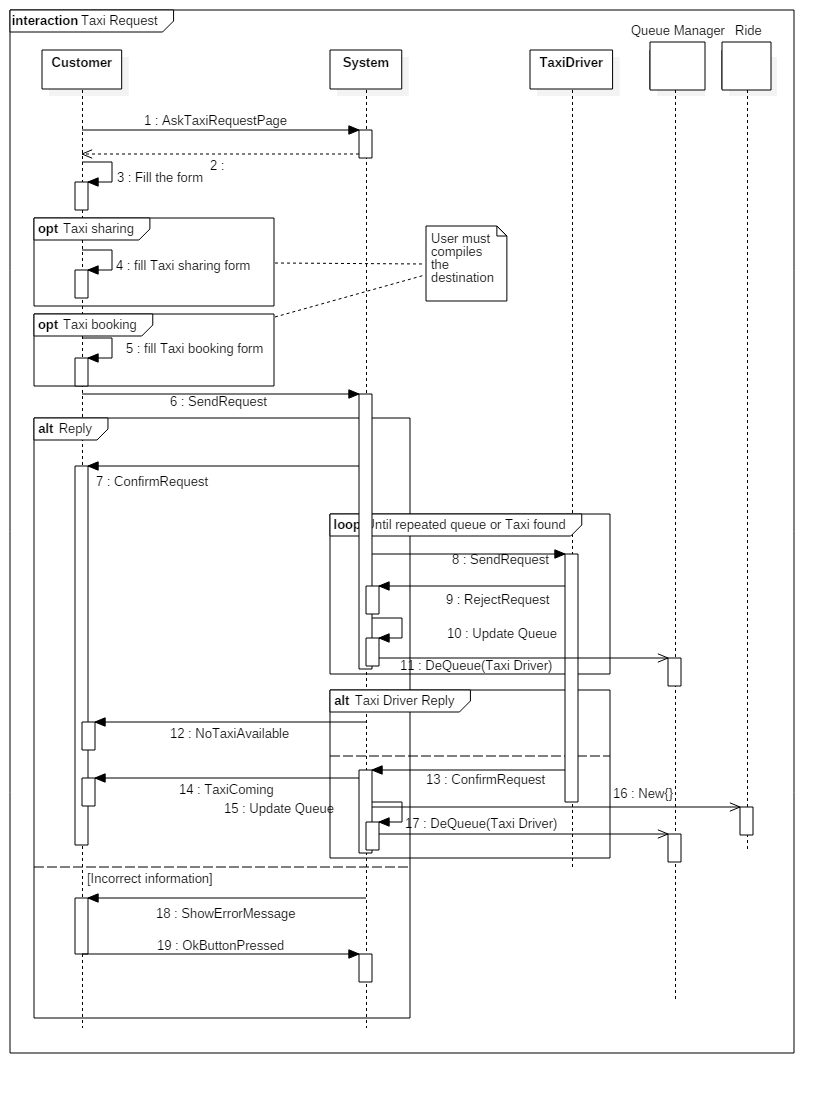
\includegraphics[width=\textwidth]{TaxiRequest}

\subsection{Manage Taxi Request}

\begin{tabular}{lp{8cm}}
\hline
Actors & Passenger \\
\hline
Preconditions &  \\
\hline
Execution Flow &  
		\begin{enumerate}
			\item The Passenger request the Taxi Request Management page
			\item The System load the page and return it to the Passenger
			\item The Passenger can modify the Request full filling the modify Request
			\item The System modify the request and return a confirm to the Passenger
			\item The Passenger can delete the request, submitting the operation to the System
			\item The System update the queue and return a confirmation to the Passenger
		\end{enumerate} 
	\\ 
\hline
Postconditions & 
	\begin{itemize}
		\item If the Passenger choose to modify the Request, the request is updated 
		\item If the Passenger choose to delete the Request, the request is canceled and the taxi is now in queue
	\end{itemize} \\
\hline
Exceptions & 
	\begin{itemize} 
		\item The Passenger provides incorrect informations in the modify request form
		\item The Passenger cancel the request too late
	\end{itemize}
\end{tabular}

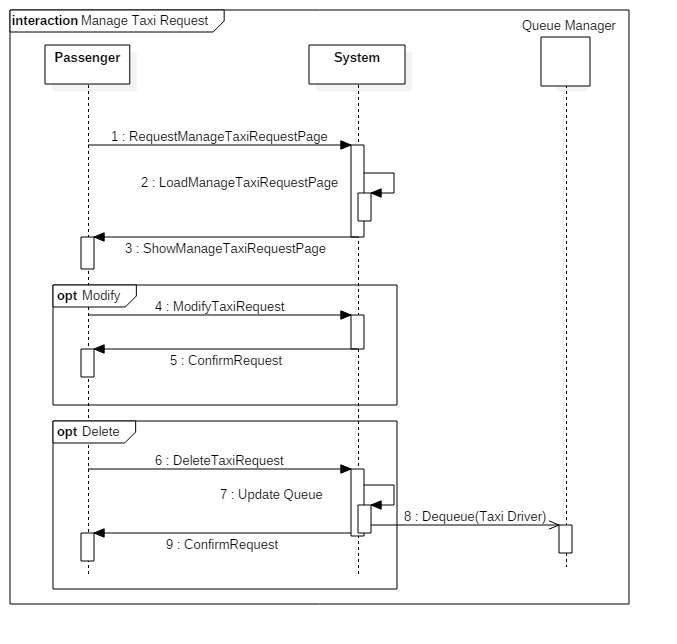
\includegraphics[width=\textwidth]{ManageTaxiRequest}

\subsection{Report Taxi}

\begin{tabular}{lp{8cm}}
\hline
Actors & Passenger \\
\hline
Preconditions & \\
\hline
Execution Flow &  
		\begin{enumerate}
			\item The Passenger request the Report Taxi page
			\item The System elaborate the request and ask to the Passenger the report information
			\item The Passenger fill the form and submit the report
			\item The System check the data obtained
			\item The System update the Taxi Driver informations
			\item The System notify to the Passenger the successful of the operation
		\end{enumerate} 
	\\ 
\hline
Postconditions & The Taxi Driver is reported by the current Passenger \\
\hline
Exceptions & The Passenger provides wrong informations in the report form
\end{tabular}

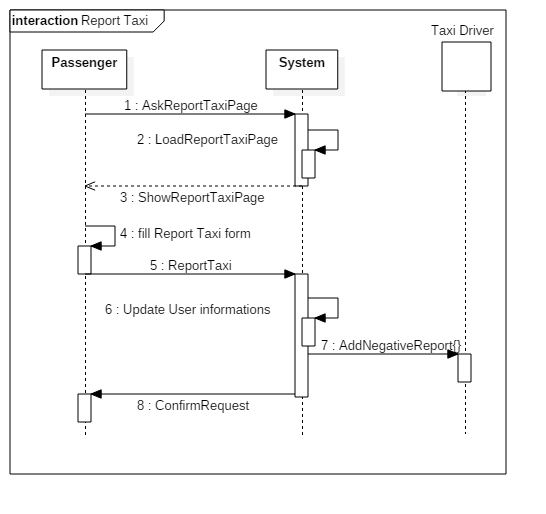
\includegraphics[width=\textwidth]{ReportTaxi}

\subsection{Report User}

\begin{tabular}{lp{8cm}}
\hline
Actors & Taxi Driver \\
\hline
Preconditions & The Taxi Driver should had carried the User past 24 hours \\
\hline
Execution Flow &  
		\begin{enumerate}
			\item The Taxi Driver request the Report User page
			\item The System elaborate the request and ask to the Taxi Driver the report information
			\item The Taxi Driver fill the form and submit the report
			\item The System check the data obtained
			\item The System update the User informations
			\item The System notify to the Taxi Driver the successful of the operation
		\end{enumerate} 
	\\ 
\hline
Postconditions & The User is reported by the Taxi Driver \\
\hline
Exceptions & The Taxi Driver provides wrong informations in the report form
\end{tabular}

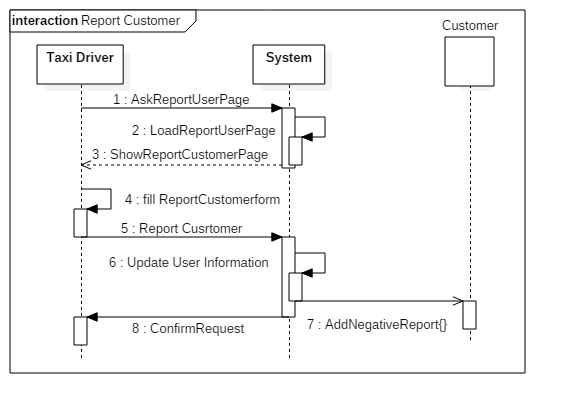
\includegraphics[width=\textwidth]{ReportUser}

\subsection{Manage Personal Informations}

\begin{tabular}{lp{8cm}}
\hline
Actors & User or Taxi Driver \\
\hline
Preconditions & \\
\hline
Execution Flow &  
		\begin{enumerate}
			\item The User (or Taxi Driver) request the User profile page
			\item The System returns the personal informations of the User (or Taxi Driver)
			\item The User (or Taxi Driver) can request the edit of the profile
			\item The System return the editable informations of the profile
			\item The User (or Taxi Driver) can edit those data and send the changes to the System
			\item The System check the correctness of the new Informations
			\item If the informations are correct send the Change Confirm to the User (or Taxi Driver), otherwise send back an error message
		\end{enumerate} 
	\\ 
\hline
Postconditions & If the User request a modify profile and submit correct informations the Profile is changed \\
\hline
Exceptions & The User provides wrong informations
\end{tabular}

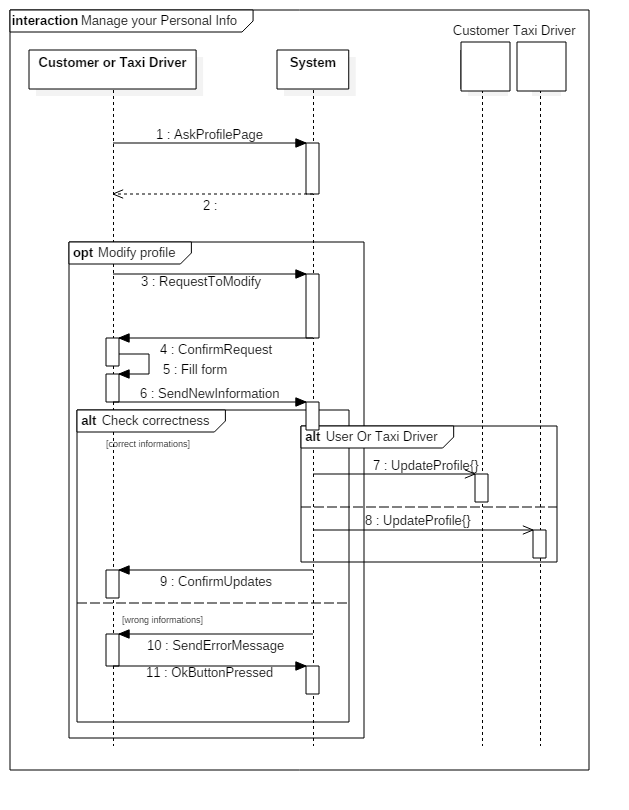
\includegraphics[width=\textwidth]{ManageInformation}

\subsection{Available}

\begin{tabular}{lp{8cm}}
\hline
Actors & Taxi Driver \\
\hline
Preconditions & \\
\hline
Execution Flow &  
		\begin{enumerate}
			\item The Taxi Driver request the Taxi profile page
			\item The System returns the personal informations of the Taxi
			\item The Taxi Driver notify the availability to the System
			\item The System update the local queue
			\item The System confirm the request to the Taxi Driver
		\end{enumerate} 
	\\ 
\hline
Postconditions & The Taxi Driver is now Available \\
\hline
Exceptions & 
	\begin{itemize} 
		\item The Taxi Driver is located in a invalid zone
		\item The Taxi Driver is carrying a Passenger
		\item The Taxi Driver is yet available
	\end{itemize}
\end{tabular}

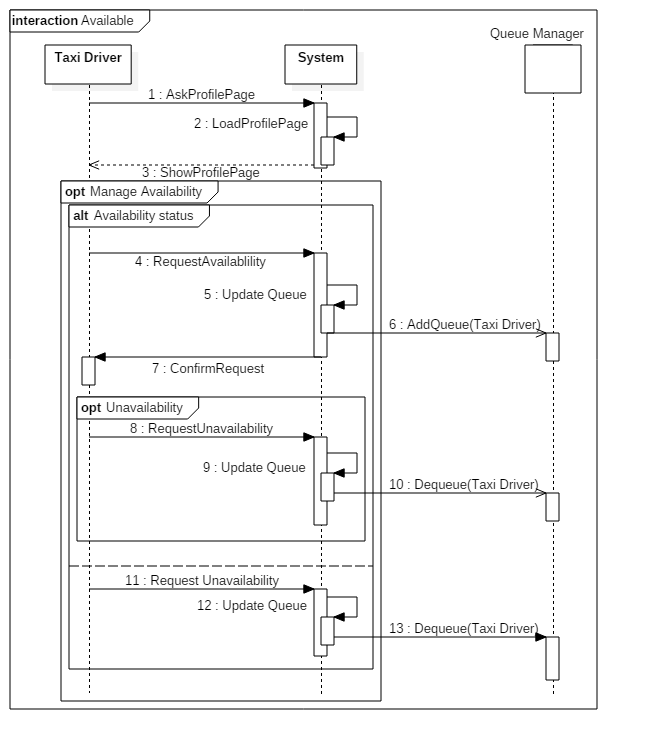
\includegraphics[width=\textwidth]{Available}

\subsection{Notify Problem}

\begin{tabular}{lp{8cm}}
\hline
Actors & Taxi Driver \\
\hline
Preconditions & The Taxi is available\\
\hline
Execution Flow &  
		\begin{enumerate}
			\item The Taxi Driver request the Report Problem page
			\item The System returns the page of the Report requiring problem informations
			\item The Taxi Driver fill the form and send the information
			\item The Taxi Driver can request another Taxi for the User who is carrying (if is carrying one)
			\item If the Taxi Driver request another Taxi the System looks for a available Taxi Driver
			\item If exist an available Taxi change the carrier of the User with the new Taxi Driver and send him, otherwise notify the unavailability
			\item The System return the success of the operation
		\end{enumerate} 
	\\ 
\hline
Postconditions & The problem is submitted into the System \\
\hline
Exceptions & 
	\begin{itemize} 
		\item The Taxi Driver is located in a invalid zone
		\item The Taxi Driver fill the form with wrong informations
	\end{itemize}
\end{tabular}

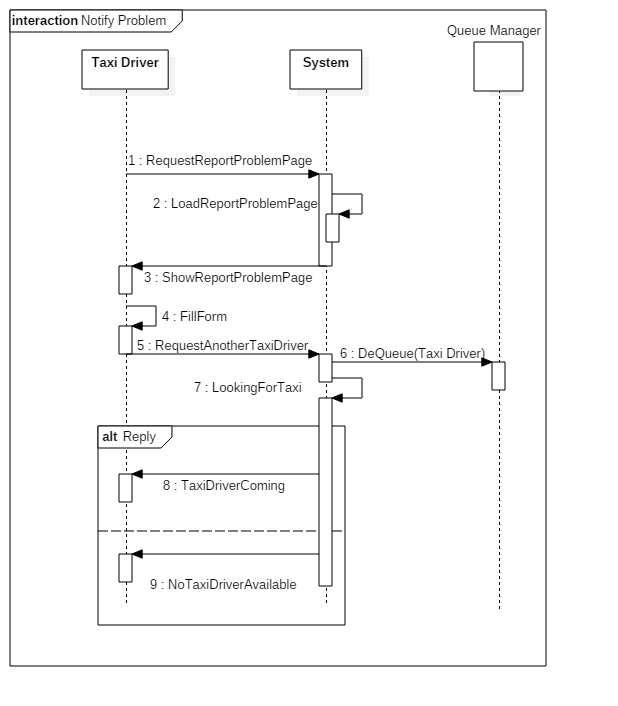
\includegraphics[width=\textwidth]{NotifyProblem}

\end{document}